% !TeX root = ../Book2.tex
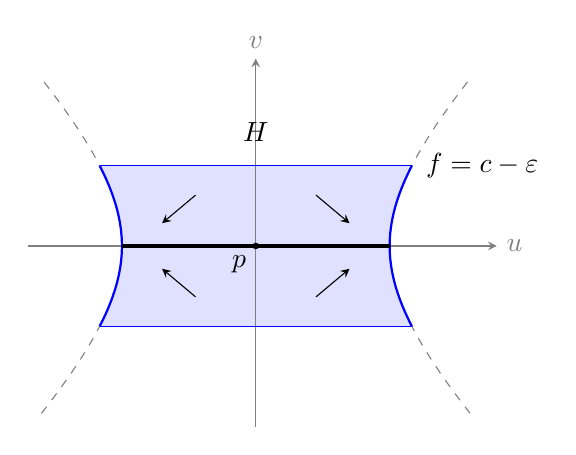
\begin{tikzpicture}[scale=1.7,>=stealth]
	\fill[blue!12] plot[domain=-.6:.6,samples=40] ({sqrt(1+\x*\x)},\x) -- plot[domain=.6:-.6,samples=40] ({-sqrt(1+\x*\x)},\x) -- cycle;
	\draw[->,gray] (-1.7,0)--(1.8,0) node[right] {\(u\)};
	\draw[->,gray] (0,-1.35)--(0,1.4) node[above] {\(v\)};
	\draw[dashed,gray] plot[domain=-1.25:1.25,samples=50] ({sqrt(1+\x*\x)},\x);
	\draw[dashed,gray] plot[domain=-1.25:1.25,samples=50] ({-sqrt(1+\x*\x)},\x);
	\draw[thick,blue] plot[domain=-.6:.6,samples=40] ({sqrt(1+\x*\x)},\x);
	\draw[thick,blue] plot[domain=-.6:.6,samples=40] ({-sqrt(1+\x*\x)},\x);
	\draw[blue] ({-sqrt(1.36)},.6)--({sqrt(1.36)},.6);
	\draw[blue] ({-sqrt(1.36)},-.6)--({sqrt(1.36)},-.6);
	\draw[very thick] (-1,0)--(1,0);
	\draw[->] (.45,.38)--(.7,.17);
	\draw[->] (-.45,.38)--(-.7,.17);
	\draw[->] (.45,-.38)--(.7,-.17);
	\draw[->] (-.45,-.38)--(-.7,-.17);
	\fill (0,0) circle (.025) node[below left] {\(p\)};
	\node at (0,.85) {\(H\)};
	\node[anchor=west] at (1.2,.6) {\(f=c-\varepsilon\)};
\end{tikzpicture}
